% Created 2014-12-23 Tue 13:46
\documentclass[11pt]{article}
\usepackage[utf8]{inputenc}
\usepackage[T1]{fontenc}
\usepackage{fixltx2e}
\usepackage{graphicx}
\usepackage{longtable}
\usepackage{float}
\usepackage{wrapfig}
\usepackage{rotating}
\usepackage[normalem]{ulem}
\usepackage{amsmath}
\usepackage{textcomp}
\usepackage{marvosym}
\usepackage{wasysym}
\usepackage{amssymb}
\usepackage{hyperref}
\tolerance=1000
\usepackage{fullpage}
\usepackage[backend=bibtex,sorting=none]{biblatex}
\usepackage{hyperref}
\usepackage{amsmath}
\usepackage{amssymb}
\addbibresource{telomeres.bib}
\author{Kyle M. Douglass}
\date{\today}
\title{Telomere Structure Estimation}
\hypersetup{
  pdfkeywords={},
  pdfsubject={},
  pdfcreator={Emacs 24.4.50.1 (Org mode 8.2.6)}}
\begin{document}

\maketitle
\tableofcontents


\section{Introduction to telomere biology}
\label{sec-1}
Telomeres consist of DNA tandem repeat sequences, their associated
binding proteins, and a non-coding RNA transcript. They are located at
the end of chromosomes and address two important problems in
eukaryotes: the end-replication problem and the end-protection
problem. A nice summary is provided in \cite{sfeir-jcellsci-2012}.

\subsection{Telomere composition and structure}
\label{sec-1-1}
In humans, the telomere tandem repeat sequence is TTAGGG. A telomere's
size lies between 5 and 15 kb in humans. A key feature of the telomere
end in all organisms is the 3' single-stranded G-rich overhang. In
mammals, these overhangs are 30-500 nucleotides long
\cite{sfeir-jcellsci-2012}.

Associated with the telomeric DNA are proteins of the shelterin
complex. Shelterin is responsible for solving the end-protection problem,
though it acts in a complicated manner.

The six known shelterin proteins are TRF1, TRF2, RAP1, TIN2, TPP1, and
POT1. TRF1 and TRF2 bind to the duplex region of the DNA; POT1 coats
the overhang with oligonucleotide/oligosaccharide binding folds. TIN2
has a bridging function since it interacts simultaneously with TRF1,
TRF2, and TPP1.

In addition to the shelterin proteins, there are telomere-associated
proteins that are recruited by shelterin to act as ``accessory
factors.''

The long non-coding RNA might be important for telomere maintenance
and function, though little is known about the underlying molecular
mechanisms.

\subsection{Telomeres and the end-replication problem}
\label{sec-1-2}
The telomerase enzyme solves the end-replication problem and helps
counteract telomere erosion. The mechanisms underlying telomere length
regulation in mammlian cells are not fully understood, though some key
factors are known.

For example, overexpressing TRF1 in cancer-derived human cells leads
to telomere shortening, whereas depleting telomeres of TRF1 results in
elongation. Reducing levels of TRF2 and TIN2 leads to telomere
extension, but also to heterochromatic marks that might offset the
extension. There are also repressive histone marks on telomeric
chromatin. Deletion of these marks correlates with large elongations
of telomeres.

\subsection{Mammalian telomeres have nucleosomes}
\label{sec-1-3}
Mammalian telomeres are enriched with repressive histone marks,
including H3K9me3 and H4K20me3 and the heterochromatin-specific
factors chromobox homolog (CBX) 1, 3, and 5. Depleting these marks
correlates with telomere elongation.

\subsection{Project goals}
\label{sec-1-4}

\begin{enumerate}
\item Establish a rigorous quantitative method for determining the size
of chromatin structures from STORM data.
\item Use the method to determine the distribution of physical telomere
sizes in Hela L(ong) and Hela S(hort) phenotypes.
\item Demonstrate how the genomic length of Hela telomeres correlates to
physical size.
\item Determine how variation of shelterin composition at the Hela
telomere affects the physical size.
\item Use the measured size distributions and polymer modeling to
estimate the degree and nature of telomere packaging.
\item Correlate changes in telomere polymeric properties to histone marks
acquired after knockdown of shelterin components.
\end{enumerate}

\section{Super-resolution imaging of telomeres}
\label{sec-2}
Telomeres in two phenotypes of Hela cells were imaged using the Biop's
N-STORM microscope. DNA FISH was used to attach 18 bp labels to the
telomeric repeats. The fluorescent label was Cy5. 3D imaging was
achieved using a cylindrical lens in the Fourier plane of the
microscope output, but the third dimension was not used in the end.

A single field of view consisted of about four cells on average and
about twenty or thirty labeled telomeres. 10,000 images were taken for
each field of view after bleaching Cy5 into its transient
off-state. Single molecule localizations were extracted from the
images using Nikon's NIS-Elements Ar software (possibly NIS-A N-STORM
Analysis as well).

\subsection{Data processing of STORM}
\label{sec-2-1}
The localization data for each field of view was analyzed by grouping
localizations into clusters using the DB-SCAN clustering
algorithm. Before performing the full analyses, we found that a
minimum number per cluster of 8 and neighborhood radius of 65 nm
sufficed to successfully identify clusters and avoid artifacts and
noise. In Fig.\ref{fig-sweep}, the number of identified clusters as a
function of DB-SCAN clustering parameters is plotted. The plateau is
the ideal area of the parameter space because neighboring telomeres
are not grouped into one cluster and sparse clusters are still
identified.

\begin{figure}[htb]
\centering
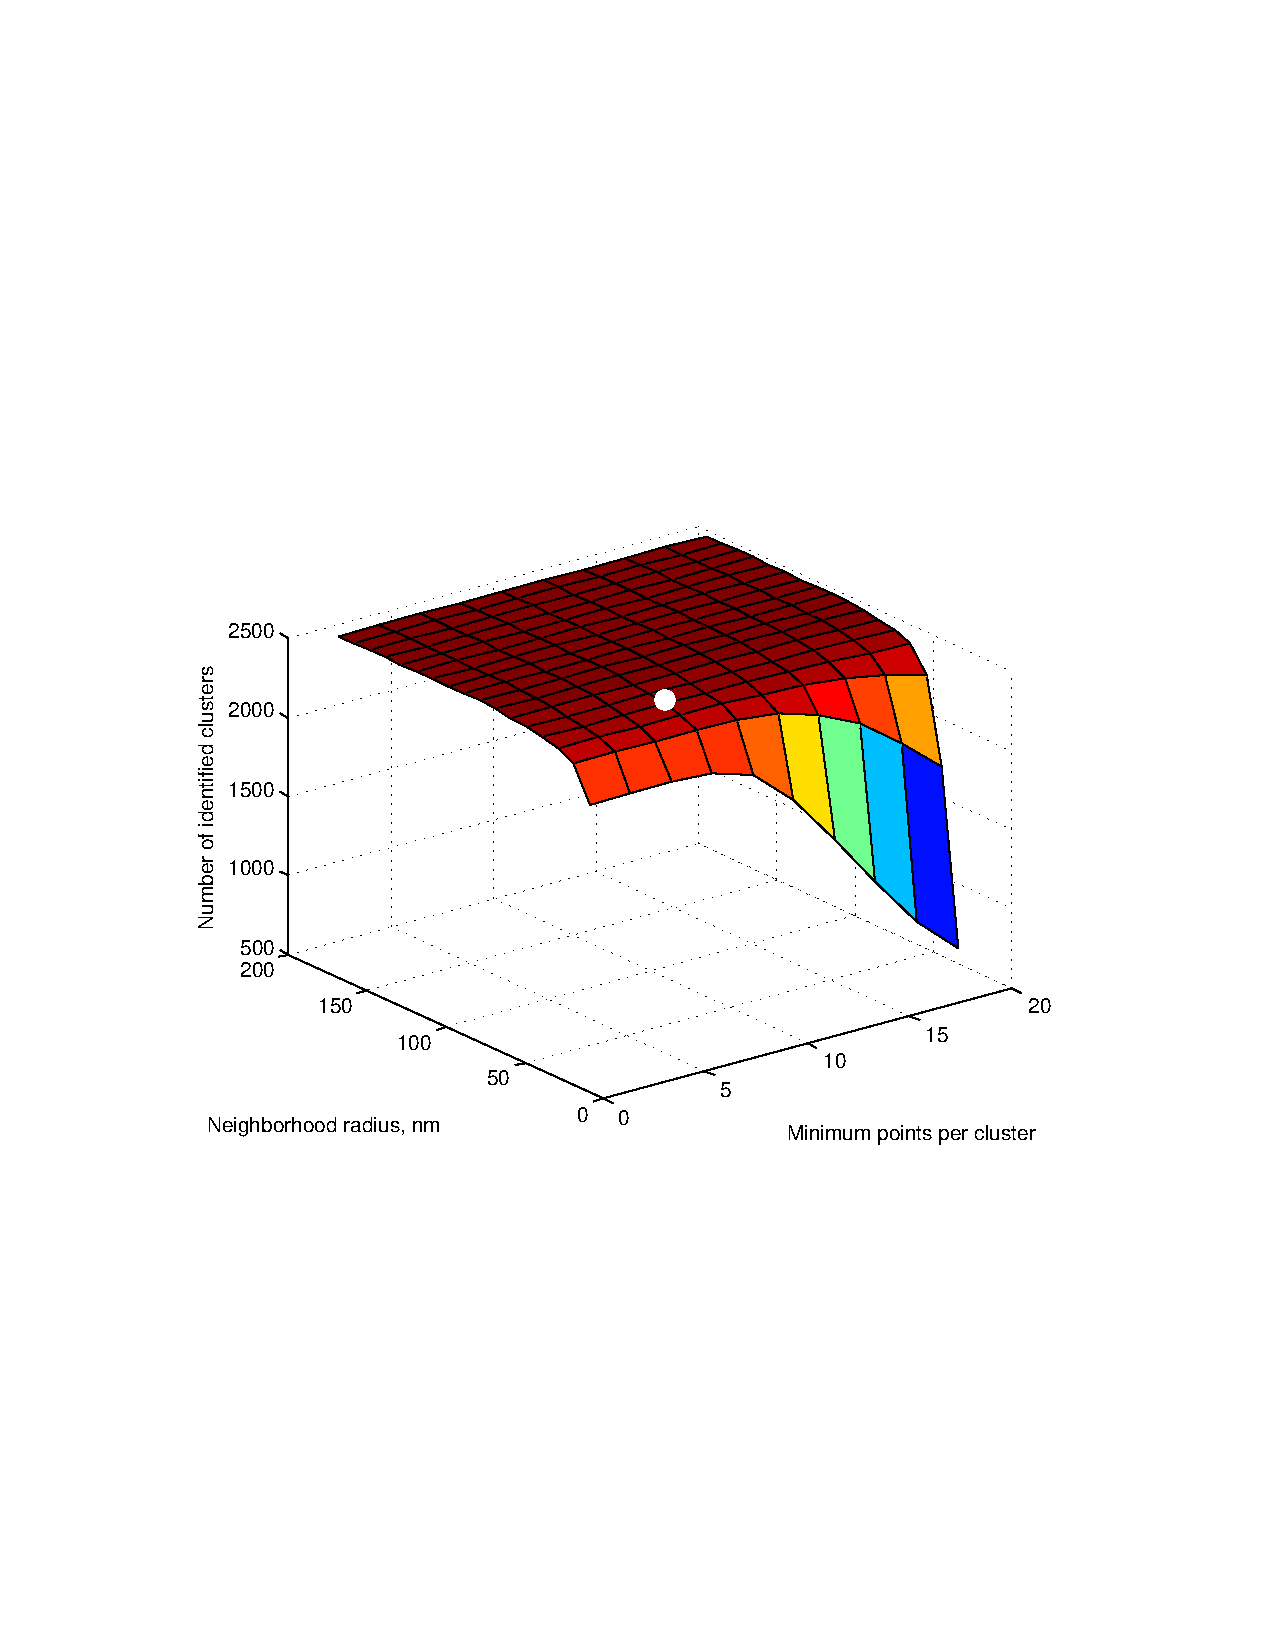
\includegraphics[width=.9\linewidth]{./images/sweep.pdf}
\caption{\label{fig-sweep}The number of identifiable clusters using DB-SCAN in the original Hela L dataset as a function of the minimum points per cluster and the neighborhood radius. The white circle marks $k = 8$ and $\epsilon = 65$, the values used in all datasets. The plateau indicates the optimum region because different telomeres are not grouped into the same cluster whereas spare clusters are still identified.}
\end{figure}

\subsection{Assessing telomere size}
\label{sec-2-2}
The properties of STORM measurements prevent the accurate
determination of any single telomere structure. The reason for this
can be seen in Fig.\ref{fig-sampling}. A small portion of the DNA
polymer is illustrated in A. However, one only has access to the data
seen in B, which represents the individual localizations found during
imaging. The localizations only reflect the true structure to a degree
due to random labeling and finite localization precisions. An
additional source of randomness comes from the fact that the telomere
genomic length is not a single number, but is also random as well. The
problem is essentially this: which of the many contours that can be
traced through the localization point data is the real chromatin
conformation? Even with extremely small localization precisions,
random labeling of the polymer would still prevent answering this
question exactly.

\begin{figure}[htb]
\centering
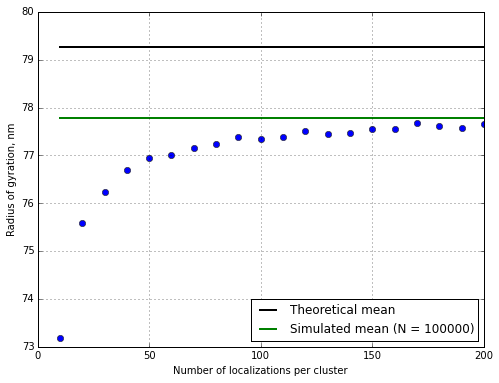
\includegraphics[width=.9\linewidth]{./images/polymer_sampling.pdf}
\caption{\label{fig-sampling}A) An illustration of a portion of telomeric DNA. B) Due to a finite localization precision and random labeling of the structure, the individual localizations only marginally reflect the underlying DNA structure.}
\end{figure}

Because the real telomere conformation cannot be determined from
STORM, we instead choose to analyze a statistical measure from the
ensemble of telomeres, the \textbf{radius of gyration, $R_g$}. This has two
advantages: 1) it satisfies our intuitive notion of size for a
polymer, and 2) the mean $R_g$ of the ensemble has an analytical
solution from polymer physics, which we can use to constrain our
models.

Note that we are not measuring \textbf{mean end-to-end distances} like in
many earlier works, (c.f. \cite{bystricky-pnas-2004}). In these works,
specific genomic sequences could be labeled and the histogram of
distances between two labeled sequences accurately determined. Because
the telomeres are genomic repeats and because of stochasiticity of the
labeling mentioned above, the radius of gyration is a more appropriate
measure of size. $R_g$ is also more amenable to assessing the telomere
structure because the genomic distances are much smaller than in
previous works (telomeres are at most 35 kb, whereas previous work
explored genomic distances on the order of 100 kb.) Genomic and
physical distances between molecules are too small to accurately
determine their separation distributions at these scales.

We should also note that the localization precision of the
measurements in the z-direction is about 50 nm. This is of the same
order of magnitude as the telomere size. For this reason, we analyze
the projected radii of gyration, i.e. the radius of gyration computed
from the localizations' x- and y-coordinates only. For a polymer in
thermodynamic equilibrium, the projected gyration radius is equal to
the true, three-dimensional gyration radius up to a constant factor of
$\sqrt{3/2}$ \cite{rivetti-jmolbiol-1996}.

\section{Polymer modeling of telomeric chromatin}
\label{sec-3}
Polymer simulations are now becoming useful tools for modeling
experimental data on chromatin and predicting other structural
features of DNA \cite{rivetti-jmolbiol-1996, giorgetti-cell-2014}.

The difference between our work and the recent chromatin simulations
of topologically associating domains (TAD's) is primarily one of
scope: in \cite{giorgetti-cell-2014}, the authors model chromatin
conformations on the 100 kb scale by allowing for independent
interaction energies between any two sections of the fiber,
essentially including the heterogeneity of the fiber as a central
aspect of their model. This is important for studying interactions
between enhancer/promoter pairs, which should have more favorable
interaction energies than with other sections of the fiber. However,
the telomeres are composed of genomic repeats and are therefore much
more homogeneous. Their smaller size also restricts the number of
conformations available for them to adopt.

For these reasons, we modeled the polymer as simpler a homogeneous
wormlike chain for which only two parameters are needed to describe
the conformational ensemble, the packing ratio $c$ and the persistence
length $\ell_p$. The packing ratio is the number of base pairs per
nanometer. To simulate a wormlike chain, we also needed the genomic
length of telomeres which, when multiplied with $c$ gives the fiber's
contour length.

\subsection{Theory of the wormlike chain and a simulation approach}
\label{sec-3-1}
In the simplest WLC model, we treat the polymer as a semiflexible and
homogeneous rod with a negligible thickness and a length $L_c$, known
as the contour length. The flexibility of the rod is described by its
persistence length $\ell_p$. Intuitively, the persistence length is
the average length over which the polymer remains approximately
straight. Polymers with a longer persistence length will be more rigid
than shorter ones.

Mathematically, the persistence length is the characteristic length
describing the exponential decay of the tanget-tanget correlation
function \cite{phillips-pbotc-2009},

\begin{equation}
  \label{eq-tantancorr}
  \left< \mathbf{t} \left( s \right) \cdot \mathbf{t} \left( 0 \right) \right> \sim \exp \left( s / \ell_p \right)
\end{equation}

where $\mathbf{t} \left( s \right)$ is the unit vector tangent to the
polymer at the one-dimensional coordinate $s$ along the polymer. For
distances $s$ much greater than $\ell_p$, \eqref{eq-tantancorr}
states that there will be no correlation in the direction that the
tangent vectors point.

The subunits that make up most polymers are very small molecules and
are thus subject to agitation by the random collisions with other
molecules in their environment. This is especially pertinent to
polymers in aqueous environments, where collisions with the solvent
molecules cause the polymer to change shape and conformation many
times a second. According to Boltzmann's statistics, the probability
that a semiflexible polymer in thermodynamic equilibrium will be found
in one of any of its possible conformations at an instant in time is
proportional to the Boltzmann factor

\begin{equation}
  \label{eq-boltzmann}
  P \left( U \right) \sim \exp \left( -\frac{U}{k_B T}\right)
\end{equation}

where $P \left( U \right)$ represents of the probability of observing
a polymer conformation with associated internal energy $U$, $k_B$ is
Boltzmann's constant and $T$ is the temperature of the system. The
fact that it takes energy to bend the polymer into a particular
conformation reflects the ``semiflexible'' qualities of the polymer.

The energy $U$ required from the environment to achieve a given
conformation can be determined by dividing the polymer into many short
sections such that it can be reprensented as the summation of the
energies of many small circular arcs. The energy required to bend a
rod through an angle $\theta$ with Young's modulus $E$, moment of
inertia $I$ is

\begin{equation}
\label{eq-bending-energy}
  U = \frac{EI}{2s}\theta^{2}
\end{equation}

The persistence length is related to the rod's mechanical properites
by \cite{phillips-pbotc-2009}

\begin{equation}
  \ell_p = \frac{EI}{k_{B}T}
\end{equation}

To simulate a wormlike chain, it suffices to create small linear
segments with angles between the segments governed the probability
distribution obtained by substituting Eq. \ref{eq-bending-energy} into
Eq. \ref{eq-boltzmann} and using the relationship above for the
persistence length. This will produce a Gaussian distribution, which
is easily sampled on a computer. To produce a 3D chain, one must also
include a random rotation of uniform probability between 0 and $2\pi$
along the axis of one of the segments. Doing so effectively extends
the simulation of 2D chains described in \cite{rivetti-jmolbiol-1996}.

\subsection{Strategy for estimating telomere polymer properties}
\label{sec-3-2}
We want to estimate the packing density $c$ and the persistence length
$\ell_p$ for the telomeres. This would allow us to quantitatively
understand how shelterin modulates their physical structures.

We have the distributions of measured 3D gyration radii for about 1000
telomeres in each of many conditions, including wild type and
shelterin knockdowns of different proteins.

Our strategy is to simulate a large number of polymers with input
parameter-pair values $\left(c, \ell_p \right)$ that we can
choose. The genomic lengths of the telomeres are constrained by the
mean genomic length and the minimum and maximum values, all three of
which can be estimated from the Southern blot data. (Gaining more
precise genomic length distribution information is not possible due to
the nature of the Southern blot measurement). After simulating each
polymer, it is ``labeled'' with flourophores whose positions have been
randomly bumped to reflect the estimated localization imprecision of
the measurement (see Fig. \ref{fig-sampling} above). The radius of
gyration for the displaced fluorophores is measured, and a probability
distribution of measured radii of gyration for all simulated and
sampled polymers is constructed.

The simulated probability distribution for every parameter pair
$\left(c, \ell_p \right)$ is then compared to the measured STORM
distribution using maximum likelihood reconstruction. The goal is to
find which pair of polymer properties was most likely to have produced
the measured dataset.

In other words, we're searching for the values of $c$ and $\ell_p$
that produce a probability distribution of gyration radii that best
matches the measured distribution.

\subsection{Preliminary results for telomere maximum likelihood reconstruction}
\label{sec-3-3}
In Fig. \ref{fig-mlr}, we plot the log-likelihood function for each
pair of values for the packing density and persistence lengths. The
redder the color, the higher the log-likelihood value, and the better
the $R_g$ distribution for that pair of parameter values matches the
measured distribution.

\begin{figure}[htb]
\centering
\includegraphics[width=.9\linewidth]{./images/mlr.pdf}
\caption{\label{fig-mlr}Log-likelihood that the simulated distribution of $R_g$ values matches the measured one from STORM. Redder colors denote higher log-likelihoods. In particular, regions near $c=30$ and $\ell_p = 50$, as well as $c=50$ and $\ell_p = 90$ match the measured data well.}
\end{figure}

There are a few things to note here: for one, contours of constant
log-likelihood are very crooked. This is actually because of
under-sampling the conformational distribution in the simulations and
because a discrete number of parameter-pair values were
simulated. 1000 conformations were simulated for each pair of
parameter values in this plot. Prior simulations with 50,000
conformations produced much smoother contours. Also, in
Fig. \ref{fig-mlrgrid}, we mark what pair of values were
simulated. Once the full parameter space is mapped like this, we can
explore the important regions by doing a finer sampling over a smaller
region.

\begin{figure}[htb]
\centering
\includegraphics[width=.9\linewidth]{./images/mlrgrid.pdf}
\caption{\label{fig-mlrgrid}Same as above, but with a grid denoting what parameter-pair values were simulated.}
\end{figure}

Importantly, the region near $c=30 \, bp/nm$ and $\ell_p = 50 \, nm$
has a high likelihood value. This means that there should be a good
overlap between the simulated $R_g$ distributions and the measured
STORM $R_g$ distributions. To show this, we plot the measured and
simulated distributions for $\ell_p = 50 \, nm$ with $c=30 \, bp/nm$
and $c=50 \, bp/nm$ in Figs. \ref{fig-distc30} and
Fig. \ref{fig-distc50}, respectively. A much better agreement between
the simulated model and the measured data is seen in the first figure.

\begin{figure}[htb]
\centering
\includegraphics[width=.9\linewidth]{./images/Probabilities_c30_lp50.png}
\caption{\label{fig-distc30}Measured and simulated $R_g$ distributions for $c=30 \, bp/nm$ and $\ell_p = 50 nm$.}
\end{figure}

\begin{figure}[htb]
\centering
\includegraphics[width=.9\linewidth]{./images/Probabilities_c50_lp50.png}
\caption{\label{fig-distc50}Measured and simulated $R_g$ distributions for $c=50 \, bp/nm$ and $\ell_p = 50 nm$.}
\end{figure}

These values allow us to make a comparison with known chromatin
models. For example, the \emph{10 nm fiber} has a packing density of 15
bp/nm and persistence length of 30 nm. The \emph{30 nm fiber} has a packing
density of 100 bp/nm and a persistence length of 200 nm. This
preliminary data suggests that the telomere packing is actually much
closer to the 10 nm fiber. Our initial estimates also show that Hela S
cells have a lower packing density than Hela L, which may be due to
the higher amounts of shelterin in Hela L. We do not yet have the
simulation results yet to show this.

\section{What's next?}
\label{sec-4}

\subsection{Refine the parameter estimations}
\label{sec-4-1}
First, we need to run the simulations with a larger number of steps
(about 100,000 compared to 1000). This will take several days, so
Christmas break is an ideal time to do this. This will allow us to
better refine the parameter space plots and identify what regions need
to be sampled with a finer grid.

We also need to determine the uncertainty in the parameter value
estimates. Judging by the extreme differences between distributions
when $c=30 \, bp/nm$ and $c=50 \, bp/nm$, it looks like the
uncertainty in the packing density is going to be small. $\ell_p$
cannot be so easily constrained, though, in part because the telomeres
are so small. The poor constraint on one parameter could be expected
since $c$ and $\ell_p$ are actually only independent parameters when
the polymer contour length is shorter than the persistence
length. When the contour length is much greater than the persistence
length, the only parameter governing polymer configuration is the
ratio $\frac{c}{\ell_p}$ \cite{martin-thesis-2008}. At this point, the
wormlike chain becomes the freely-jointed chain.

One way to address uncertainty in maximum likelihood estimates is to
compute the local curvature of the parameter space at the point of the
best estimate. This involves taking the second derivative of the
parameter space and requires a finely sampled grid at the maximum. Due
to the prohibitive computation times involved, we're delaying this
uncertainty estimation for now and instead looking at the overlap
between measured and simulated distributions to qualitatively judge
the uncertainty in the parameters.

\subsection{Improve simulation speeds}
\label{sec-4-2}
A portion of the simulation code can be rewritten to utilize parallel
processing. On my 12-core machine, this should result in a 12-times
reduction in the computation time. This isn't so important now and
will likely be done after the break, since I can get a number of
simulations to finish with the current code over Christmas.

\subsection{Compare parameter value estimations for Shelterin knockdowns}
\label{sec-4-3}
We've observed that the mean radius of gyration is always smaller when
TRF2 is knocked down. There is also a larger number of heterochromatic
marks on the telomeres in TRF2 knockdowns, which suggests that charge
screening on the histones should result in telomere compaction. In
Fig. \ref{fig-trfKDs}, we show measured mean gyration radii for TRF1,
TRF2, and TRF1/TRF2 double knockdowns, compared to the control
pSuper. It also intersting to note that TRF1 knockdowns result in
telomere decompaction, which might be seen in the figure as well,
though the results are less obvious and the cause less clear
\cite{sfeir-jcellsci-2012}.

\begin{figure}[htb]
\centering
\includegraphics[width=.9\linewidth]{./images/sizes-TRF12.png}
\caption{\label{fig-trfKDs}Mean gyration radii for the TRF1, TRF2, and TRF1/TRF2 knockdown experiments. The control is pSuper. Error bars are standard errors of the mean.}
\end{figure}

We would like to quantitatively assess exactly how much more compact
the TRF2 knockdowns are than the controls, which is reflected in the
value for the packing density. At this point, though, it's unclear
whether we can say that there is a statistically significant
difference in packing densities since the change in mean size is
rather small.

If we are however capable of determining the change in packing
density, this will be the first physical measurement (to my knowledge)
of small scale compaction in chromatin due to heterochromatic marks
that are caused by charge screening on the histones.

\section{Additional features not included in the model}
\label{sec-5}

\subsection{Excluded volume interactions}
\label{sec-5-1}
The polymer/STORM model I've developed does not take into account
excluded volume interactions, though these have been suggested to be
important for some chromatin fiber interactions.

The reason for this is that excluded volume interactions would require
an additional parameter in the model, which is the radius of the
excluded volume around a polymer segment. However, I know of no
constraints on this value that we can use, except for maybe the known
diameter of the 10 nm and 30 nm fibers. This is a poor constraint
because it only reflects hard-core electrostatic interactions, not the
the longer-range interactions that would more likely determine the
polymer conformation.

I also have good reason to think that excluded volume interactions are
not going to matter in telomeres anyway. We're finding a minimum
persistance length consistent with the data of about 50 nm. Since the
telomeres are only about 200 nm in diameter, the chromatin fiber
probably doesn't bend over onto itself in this condition because it's
too stiff, and thus there simply aren't enough conformations in the
ensemble where the fiber overlaps itself.

\subsection{T-loops}
\label{sec-5-2}
We are not including the T-loop in the polymer model. The T-loop is a
structure where the single strand overhang folds back and inserts
itself into the double-stranded portion of the telomere. I have been
told that these have only been observed in vitro (c.f. the work from
Prof. Zhuang's lab \cite{doksani-cell-2013}, where they isolated
telomeres and spread them out on a surface before
imaging). Additionally, our biology colleagues seem to think the
T-loop is some sort of fascination of other groups and that their
existence is in vivo is questionable.

I think it might be challenging to address this point. Our results
might in fact conflict with \cite{doksani-cell-2013} since we see a
shrinking telomere when TRF2 is knocked down. They see in vitro that
the T-loop is not formed when TRF2 is knocked down, and I suspect
(though on very limited grounds) that T-loop removal in vivo would
cause an increase in telomere size. This point really needs to be
thought about before we submit, but I haven't received much help on
this point.

\subsection{G-quadruplex}
\label{sec-5-3}
There is a higher-order structure in the telomere called a
G-quadruplex \cite{ray-pnas-2014}. It is formed by interactions
between guanines in double stranded DNA. My limited knowledge on the
subject is that the 4-guanine interaction is weak, that G-quadruplex
existence is questionable by some in vivo, and that the relatively
harsh conditions of FISH preparation would essentially remove these
formations during labeling, if they did indeed exist.

Still, we also have to address this point, like the T-loops. One way
is to suggest that the estimated packing density $c$ effectively
includes contributions from the G-quadruplexes. After all, we measure
a packing density that's higher than the 10 nm fiber; this increase
could reflect more compaction due to the formation of G-quadruplexes.


\printbibliography
% Emacs 24.4.50.1 (Org mode 8.2.6)
\end{document}
